\chapter{Console application}
\renewcommand{\baselinestretch}{\mystretch}
\label{chap:Console}
%\setlength{\parindent}{0pt}

\section{Implementation}

A Command-line User Interface (CUI) version of Vixen, named \texttt{VixenConsole}, was implemented for Linux based platforms. It is easier to operate and manage a CUI based program through remote connection instead of a distorted partially functional GUI application. \cref{chap:Guide} listed the detailed usage description of \texttt{VixenConsole}.

The original core codebase from \texttt{Vixen.dll} was used in this program with some necessary modifications. Instead of full initialisation from Vixen GUI application, only minimal initialisation of output controllers will be done from \texttt{VixenConsole} to reduce overheads. In this way, the code for the playback engine, module and data loading is still shared with the Vixen GUI application, including future improvements and patches.

\texttt{VixenConsole} reads configurations from the same location as Vixen application, the \texttt{Vixen 3} folder from user home directory. All configurations are stored as XML files, exported directly from settings object using XML serialiser. The ability to list available controllers and their configurations were added to \texttt{VixenConsole}. However, configuration modification was not yet possible from \texttt{VixenConsole}, due to the complexity of supporting every types of configuration fields within the project time constraint. To create or modify the configuration, the Vixen GUI application can be used from a computer running Microsoft Windows. Editing the XML configuration files directly using text editors is also possible.

The \texttt{FMOD} plugin used by the Vixen GUI application was outdated, no longer available for download. Therefore, audio playback using the ``Raw'' sequence was unsupported by \texttt{VixenConsole}.

\texttt{Use crontab instead of a built-in show scheduler}

\section{Loading performance}

On an embedded platform with limited computation power, the loading time of \texttt{VixenConsole} and all controller modules can take a significant time. The implemented \texttt{tidy} operation can reduce a small portion of the loading time, by remove unused settings for elements and filters. It also reduces the size of XML settings file.

However, it still takes more than 2 minutes from starting \texttt{VixenConsole} to rendering on the Noah NP1380 platform. This loading time is for the mono runtime to preform some necessary tasks such as dynamic recompile, thus unavoidable.

\section{Execution performance}

\fref{fig:raw-seq-p-c} compares the performance between \texttt{VixenLinky} and \texttt{VixenConsole} on multiple platforms. The performance comparison was done by unlimit the playback and controller refresh rate separately using both \texttt{VixenLinky} and \texttt{VixenConsole} applications, a total number of 4 tests on each of the platforms. The refresh rate data over the entire sequence time then summarised to a five-number summary representation, i.e. sample minimum, lower quartile, median, upper quartile and sample maximum. The mean values were also plotted as points. The refresh rate axis is log scale, to focus on the lower performance figures over all platforms.

\begin{figure}[t]
  \centering
  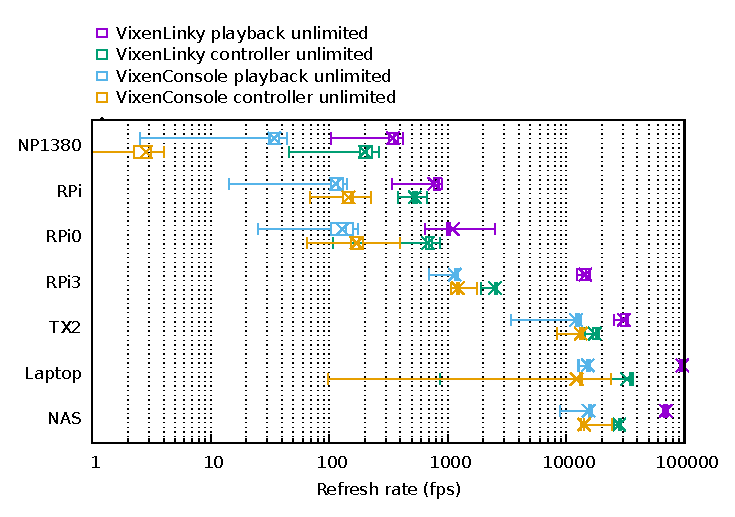
\includegraphics[width=0.9\textwidth]{Figs/raw-seq-p-c.eps}
  \caption{\footnotesize Performance comparison between \texttt{VixenLinky} and \texttt{VixenConsole}}
  \label{fig:raw-seq-p-c}
\end{figure}

By separating playback and controller update tests, the two major performance limitation factors of file IO and processing power can be separately tested.

The figure shows, \texttt{VixenConsole} runs a few times slower than the minimal implementation \texttt{VixenLinky}. On NP1380, the controller refresh rate drops below 10 fps, unusable for a 50 fps sequence. It still performs adequately on Raspberry Pi B+, both the maximum possible playback and controller refresh rate were significantly higher than 50 fps.

The mono profiler was used in an attempt to determine the most time consuming code segment on Raspberry Pi. However, it was not particularly useful. As shown by \lref{lst:mono_sample}, the information given by the profiler does not give notable highlight for performance optimisation opportunity. Apart from unhelpful unknown methods, the thread sleeping method, file reading methods and update methods are all just as expected. Some overheads from copying command arrays do show up on the summary as array coping functions, but they are unavoidable for controller module interface compatibility.

\begin{lstlisting}[float,floatplacement=ht,language=,label=lst:mono_sample,captionpos=b,caption={\footnotesize Summary of time spent in each method collected by mono profiler}]
Method call summary
Total(ms) Self(ms)      Calls Method name
  796551   796551      19237 (wrapper managed-to-native) System.Threading.Thread:SleepInternal (int)
  516874   516771       3785 (wrapper managed-to-native) System.IO.InotifyWatcher:ReadFromFD (intptr,byte[],intptr)
 1646781   412701      58603 unknown method 0xffffffffb2b3bb88
33649154   137328      58651 VixenModules.Output.TCPLinky.TCPLinky:UpdateState (int,Vixen.Commands.ICommand[])
   94269    57976      18249 Vixen.Sys.Playback:ReadFrame ()
   37151    37151     188864 (wrapper managed-to-native) object:__icall_wrapper_ves_icall_array_new_specific (intptr,int)
   31689    31689      47264 (wrapper managed-to-native) System.IO.MonoIO:Read (intptr,byte[],int,int,System.IO.MonoIOError&)
   27701    27701     123629 (wrapper managed-to-native) System.Array:FastCopy (System.Array,int,System.Array,int,int)
15553611    21874       8829 unknown method 0x102b29cc0
 9115056    20593      58659 unknown method 0xffffffffb2b38660
   22427     9027     387111 System.Diagnostics.Stopwatch:get_ElapsedMilliseconds ()
   13421     8374     387116 System.Diagnostics.Stopwatch:get_ElapsedTicks ()
43869866     7960      58635 Vixen.Sys.Output.OutputController:Update ()
    7604     7604     565017 (wrapper managed-to-native) System.Diagnostics.Stopwatch:GetTimestamp ()
    6167     6167       3020 (wrapper managed-to-native) System.Runtime.CompilerServices.RuntimeHelpers:SufficientExecutionStack ()
 4779217     5777       8845 unknown method 0x102263018
 2615069     4814      17466 unknown method 0x102264df8
    4509     4509       8821 (wrapper managed-to-native) System.Net.Sockets.Socket:Send_internal (intptr,byte[],int,int,System.Net.Sockets.SocketFlags,int&,bool)
\end{lstlisting}
